\subsection{Canais Z em cascata}

\begin{questions}
\question{
Considere a cascata de dois canais Z, conforme ilustrado na figura abaixo.
  \begin{figure}[h!]
  \centering
  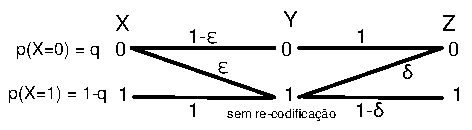
\includegraphics[width=0.55\textwidth]{../images/canalzc.pdf}
  \label{fig:canalzc}
  \end{figure}
  A saída de um canal é inserida diretamente no canal seguinte, sem recodificação.
  Encontre as probabilidades de transição do canal final criado pela cascata dos
  2 canais Z.

\begin{parts}
\part Encontre as probabilidades de transição para o canal final (entre $X$ e $Z$).
\part Encontre o valor de $\delta$ (em termos de $\epsilon$) que faz com que o canal final $XZ$
  seja simétrico e encontre a capacidade deste canal $C_{XZ}$.
\part Considere agora que, em $Y$, seja possível decodificar e recodificar a sequência recebida.
  Qual é a capacidade do sistema agora?
\end{parts}
}

\begin{solution}
\begin{parts}
\part 
  O canal efetivo entre $X$ e $Z$ é descrito pelas probabilidades
  \begin{equation}
  p(Z=0|X=0) = (1-\epsilon) + \epsilon \delta
  \end{equation}
  \begin{equation}
  p(Z=1|X=0) = \epsilon (1-\delta)
  \end{equation}
  \begin{equation}
  p(Z=0|X=1) = \delta
  \end{equation}
  \begin{equation}
  p(Z=1|X=1) = 1-\delta
  \end{equation}

  \begin{equation}
  p(z|x) = 
    \begin{pmatrix}
    (1-\epsilon) + \epsilon \delta & \epsilon (1-\delta) \\
    \delta      & 1-\delta
    \end{pmatrix}
  \end{equation}


\part
  Devemos ter $p(Z=1|X=0) = p(Z=0|X=1)$, ou seja,
  \begin{equation}
  \epsilon = \frac{\delta}{1-\delta}
  \end{equation}
  Note que esta escolha levará também a $p(Z=1|X=1) = p(Z=0|X=0)$.

  Como o canal é simétrico, teremos
  \begin{eqnarray}
  C &=& \log \vert \mathcal{Z} \vert - H(r) \nonumber \\
        &=& \log 2 - H(\delta) \nonumber \\
        &=& 1 - H(\delta).
  \end{eqnarray} 
  onde $r$ é uma linha da matriz de transição, ou seja, $r = [\delta \quad (1-\delta)]$, utilizando 
  $\epsilon = \delta / (1 - \delta)$.

\part 
  \begin{equation}
  C = \min (C_Z , C_{YZ}) .
  \end{equation}
  onde $C_Z$ é a capacidade do canal $X \text{\textemdash} Y$ e $C_{YZ}$ é a capacidade do canal $Y \text{\textemdash} Z$.

\end{parts}


\end{solution}
\end{questions}
